
%(BEGIN_QUESTION)
% Copyright 2006, Tony R. Kuphaldt, released under the Creative Commons Attribution License (v 1.0)
% This means you may do almost anything with this work of mine, so long as you give me proper credit

Følgende diagram viser en pneumatisk \textit{momentbalansert} differansetrykktransmitter, lik Foxboro modell 13A.  Begrepet ``moment'' viser til at en kraft virker på en arm og skaper et dreiemoment.  ``Momentbalanse'' er mer presist enn ``kraftbalanse'' her, fordi mekanismen balanserer moment mot moment, ikke kraft mot kraft direkte:

$$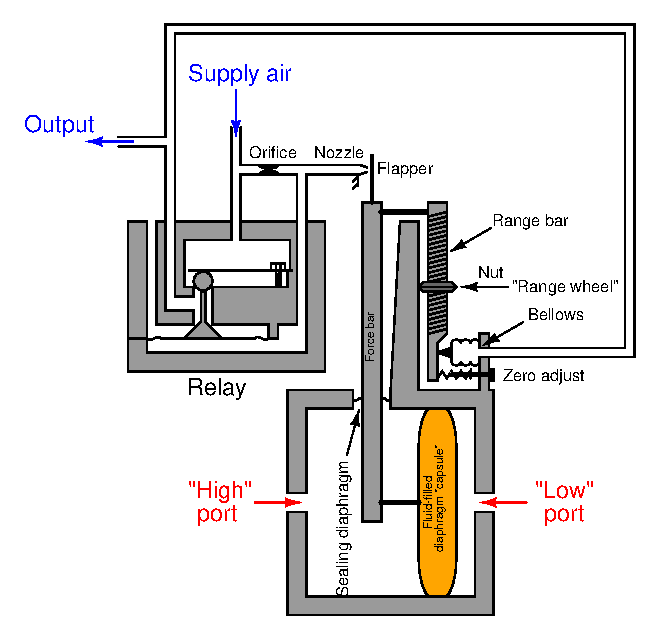
\includegraphics[width=15.5cm]{i00205x01.eps}$$

Beskriv steg for steg hvordan instrumentet responderer på økende differansetrykk (økt trykk på ``High''-siden med konstant ``Low''-side, eller redusert trykk på ``Low'' med konstant ``High'').

\vskip 20pt \vbox{\hrule \hbox{\strut \vrule{} {\bf Suggestions for Socratic discussion} \vrule} \hrule}

\begin{itemize}
\item{} Beskriv hensikten med \textit{tettemembranen} omtrent midt på kraftstangen.
\item{} Forklar hvordan instrumentet reagerer ved blokkering i følgende steder:
\begin{itemize}

\item{} Dyse
\item{} Vent (på reléhuset)
\end{itemize}
\end{itemize}

\underbar{file i00205}
%(END_QUESTION)





%(BEGIN_ANSWER)

Når differansetrykket øker (``high'' øker relativt til ``low''):

\begin{itemize}
\item{} Membrankapselen presses mot høyre.
\item{} Kraftstangen roterer mot klokka rundt tettemembranen, som virker som vippepunkt.
\item{} Bafflen nærmer seg dysen.
\item{} Dysebaktrykket øker.
\item{} Økt dysebaktrykk presser relémembranen opp.
\item{} Inne i reléet åpner kuleformet forsyningsventil og konisk ventilasjonsventil lukker.
\item{} Reléutgangstrykket øker (mer enn dysebaktrykket, på grunn av forsterkning).
\item{} Dette utgangstrykket går til belgen, som presser mot venstre i nedre ende av range bar.
\item{} Range bar roterer med klokka rundt ``range wheel'' (flyttbar fulkrummutter).
\item{} Toppen av range bar beveger seg mot høyre og trekker i kraftstangen slik at bafflen flyttes bort fra dysen.
\item{} Systemet når likevekt når kraften fra belgen via range bar balanserer kraften fra membrankapselen via kraftstangen.
\end{itemize}

Sluttresultat: utgangstrykket blir en proporsjon (faktor eller brøk) av differansetrykket over membrankapselen.

%(END_ANSWER)





%(BEGIN_NOTES)


%INDEX% Measurement, pressure: Foxboro 13A pneumatic D/P cell

%(END_NOTES)

